\setAuthor{Andres Põldaru}
\setRound{piirkonnavoor}
\setYear{2016}
\setNumber{G 10}
\setDifficulty{7}
\setTopic{Termodünaamika}

\prob{Veesoojendi}
Veesoojendis võimsusega $P=\SI{2.0}{kW}$ on algselt vesi massiga $m_0$ temperatuuril $T_0=\SI{20}{\degreeCelsius}$. Soojendisse voolab ühtlasel kiirusel juurde vett temperatuuril $T_0$ nii, et ajaühikus lisanduva vee mass $\mu=\const$. Soojendi saab täis ja vett hakkab üleval olevast avast välja voolama. Temperatuur jätkab tõusmist, stabiliseerudes \SI{36}{\degreeCelsius} juures. Soojendis oleva vee temperatuurigraafik on toodud allpool. Leidke $m_0$ ja $\mu$. Eeldage, et peale väljavoolava vee muid soojuskadusid pole ja soojendis olev vesi on alati ühtlase temperatuuriga. Vee erisoojus $c=\SI{4.2}{\frac{kJ}{kg\cdot K}}$.

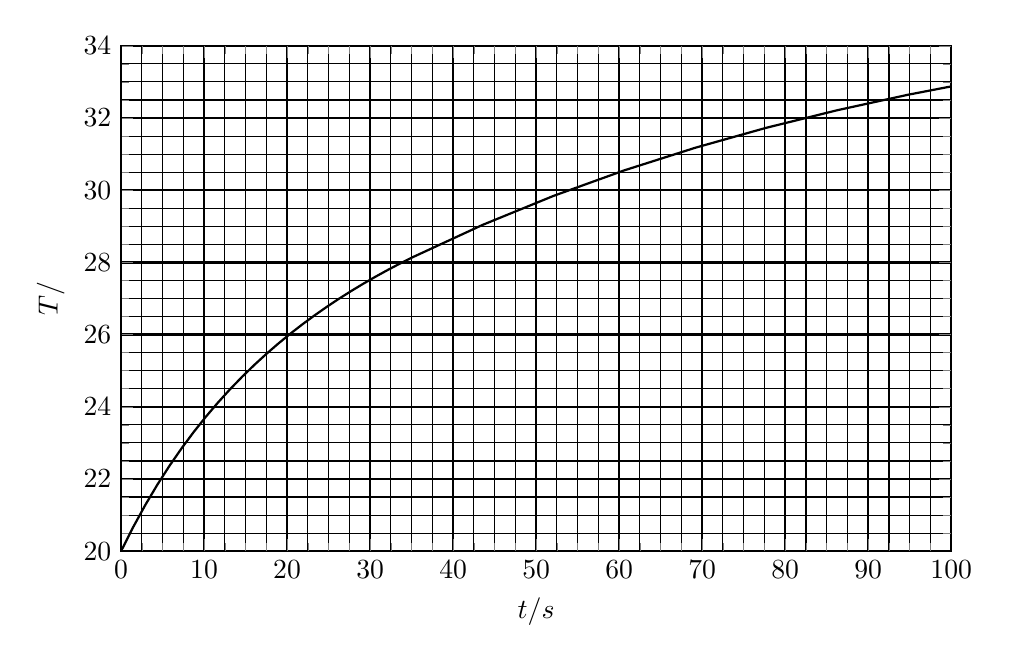
\begin{tikzpicture}
	\begin{axis}[ 
		xlabel={$t/s$},
		width = \textwidth,
		height = 8 cm,
		ylabel={$T/\si{\degreeCelsius}$},
		xmin=0, xmax = 100,
		ymin=20, ymax = 34,
		xtick distance = 10,
		ytick distance = 2,
		minor x tick num = 3,
		minor y tick num = 3,
		grid = both,
		minor grid style = {black},
		major grid style = {black, thick},
	] 
	\addplot [domain=0:35, thick]{20 + 2000/(4200*0.03)*(1-1/(1+0.03*x))};
	\addplot [domain=35:240, thick]
	{2000/(4200*0.03)+20+(20+ 2000/(4200*0.03)*(1-1/(1+0.03*35))
		-2000/(4200*0.03)-20)*e^(-0.03*(x-35)/(1+0.03*35))};
	\end{axis}
\end{tikzpicture}

\hint
Alguses on lisanduva vee temperatuur võrdne soojendis oleva vee temperatuuriga ja vett välja ei voola; seega muutub vee temperatuur ainult soojendilt saadava soojuse tõttu. Stabiilsel temperatuuril on ajaühikus väljavoolava vee soojendamiseks kulunud energia võrdne soojendi võimsusega.

\solu
Alguses on lisanduva vee temperatuur võrdne soojendis oleva vee temperatuuriga ja vett välja ei voola; seega muutub vee temperatuur ainult soojendilt saadava soojuse tõttu: $\Delta Q = c m_0 \Delta T = P \Delta t$. Kui ajahetk $\Delta t$ on piisavalt väike, saame tõusu $\Delta T / \Delta t \approx \SI{0,45}{\degreeCelsius\per\second}$, mis tuleb graafikult mõõta ajahetkel $t=0$. Tõusu saab leida, tõmmates graafikul puutuja ajahetkel $t=0$, mis läbib ligikaudu punkti $T=\SI{24.5}{\degreeCelsius}$ ja $t = \SI{10}{\second}$. Massiks saame:
$$m_0 = \frac{P}{c \frac{\Delta T}{\Delta t}} \approx \frac{\SI{2000}{W}}{\SI{4200}{\joule \per \kilogram \per \degreeCelsius}\times\SI{0,45}{\degreeCelsius\per\second}} \approx \SI{1.1}{kg}.$$

Stabiilne temperatuur saavutatakse siis, kui ajaühikus väljavoolava vee soojendamiseks kulunud energia on võrdne soojendi võimsusega. Sellest saame seose $P=\mu c(T-T_0)$, kust võttes stabiilseks temperatuuriks $T=\SI{36}{\degreeCelsius}$, saame voolukiiruseks:
$$\mu = \frac{P}{c(T-T_0)} \approx \frac{\SI{2000}{W}}{\SI{4200}{\joule \per \kilogram \per\degreeCelsius}\times \SI{16}{\degreeCelsius}} \approx \SI{0.03}{\kilogram\per\second}=\SI{30}{\gram\per\second}.$$

\probeng{Water heater}
In a water heater of power $P=\SI{2.0}{kW}$ there is initially water of mass $m_0$ and of temperature $T_0=\SI{20}{\degreeCelsius}$. Additional water with a temperature $T_0$ is flowing with even speed into the heater so that the mass of the additional water per unit of time is $\mu=\const$. The heater is filled with water and the water starts to flow out of the opening on top. The temperature continues to rise, stabilizing at $\SI{36}{\degreeCelsius}$. The temperature graph of the water in the heater is shown below. Find $m_0$ and $\mu$. Assume that besides the water flowing out of the heater there are no heat losses and that the water in the heater is always with even temperature. The specific heat of water is $c=\SI{4.2}{\frac{kJ}{kg\cdot K}}$.\\
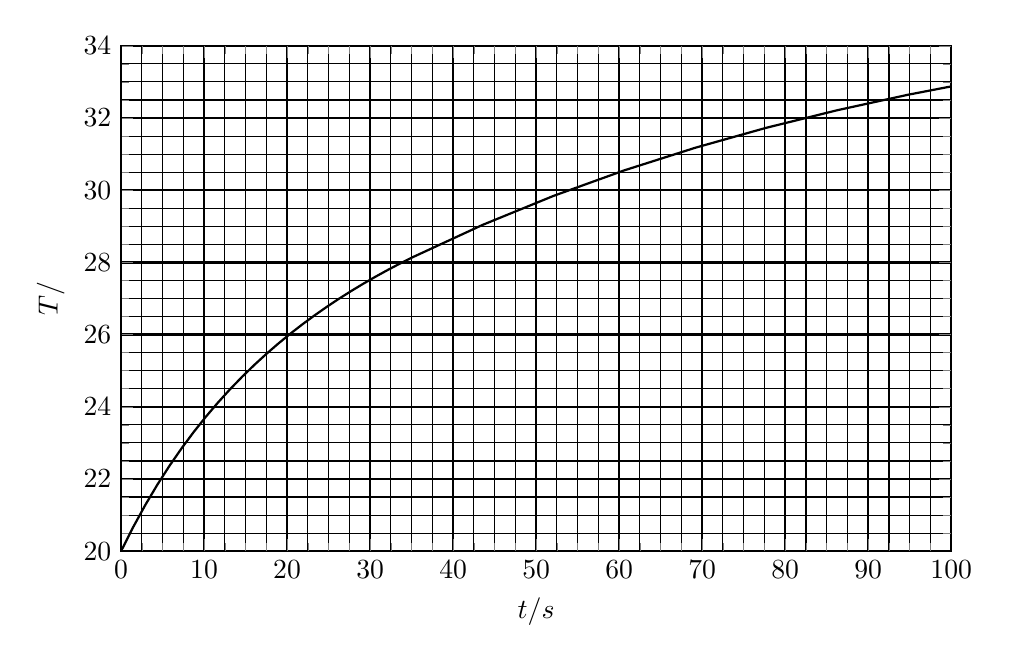
\begin{tikzpicture}
	\begin{axis}[ 
		xlabel={$t/s$},
		width = \textwidth,
		height = 8 cm,
		ylabel={$T/\si{\degreeCelsius}$},
		xmin=0, xmax = 100,
		ymin=20, ymax = 34,
		xtick distance = 10,
		ytick distance = 2,
		minor x tick num = 3,
		minor y tick num = 3,
		grid = both,
		minor grid style = {black},
		major grid style = {black, thick},
	] 
	\addplot [domain=0:35, thick]{20 + 2000/(4200*0.03)*(1-1/(1+0.03*x))};
	\addplot [domain=35:240, thick]
	{2000/(4200*0.03)+20+(20+ 2000/(4200*0.03)*(1-1/(1+0.03*35))
		-2000/(4200*0.03)-20)*e^(-0.03*(x-35)/(1+0.03*35))};
	\end{axis}
\end{tikzpicture}

\hinteng
At first the temperature of the additional water is equal to the temperature of the water in the heater and no water flows out; thus the temperature of the water only changes from the heat gotten from the heater. At a stable temperature the energy that goes to heating the amount of water flowing out per unit of time is equal to the power of the heater.

\solueng
Initially the temperature of the additional water is equal to the water temperature inside the heater and no water flows out; therefore the water temperature only changes due to the heat gotten from the heater: $\Delta Q = c m_0 \Delta T = P \Delta t$. If the moment of time $\Delta t$ is small enough then we get a slope $\Delta T / \Delta t \approx \SI{0,45}{\degreeCelsius\per\second}$ that has to be measured in the graph at a moment of time $t=0$. The slope can be found by drawing a tangent line in the graph at the initial moment of time $t=0$ which approximately goes through the point $T=\SI{24.5}{\degreeCelsius}$ and $t = \SI{10}{\second}$. We get a mass:
$$m_0 = \frac{P}{c \frac{\Delta T}{\Delta t}} \approx \frac{\SI{2000}{W}}{\SI{4200}{\joule \per \kilogram \per \degreeCelsius}\times\SI{0,45}{\degreeCelsius\per\second}} \approx \SI{1.1}{kg}.$$
A stable temperature is achieved when the energy that is necessary to heat the water flowing out per unit of time is equal to the power of the heater. From this we get a relation $P=\mu c(T-T_0)$ where if we choose the stable temperature to be $T=\SI{36}{\degreeCelsius}$ then we get the mass flow rate:
$$\mu = \frac{P}{c(T-T_0)} \approx \frac{\SI{2000}{W}}{\SI{4200}{\joule \per \kilogram \per\degreeCelsius}\times \SI{16}{\degreeCelsius}} \approx \SI{0.03}{\kilogram\per\second}=\SI{30}{\gram\per\second}.$$
\probend